\chapteropen{Chapter 16: AI engineering and agentic systems}{chapter-16}
\markboth{Ch. 16 | AI systems}{}


\begin{studycolumns}
\vspace{0pt}
\begin{eli5box}
Treat an LLM like a fluent assistant who can still misunderstand the task. It can suggest code, tests or tags, but another part of the system must check the result. Asking the assistant to promise 'I am correct' is not the same as measuring correctness.
\end{eli5box}
\textbf{Answer check:} Separate LLM proposals from deterministic validators, policy gates and execution. Valid JSON can still have a wrong shape, disallowed tags or too many tags. An LLM-selected role does not authenticate a user; agent agreement does not prove passing tests.
\end{studycolumns}


\par\smallskip\noindent\begin{minipage}{\linewidth}\centering
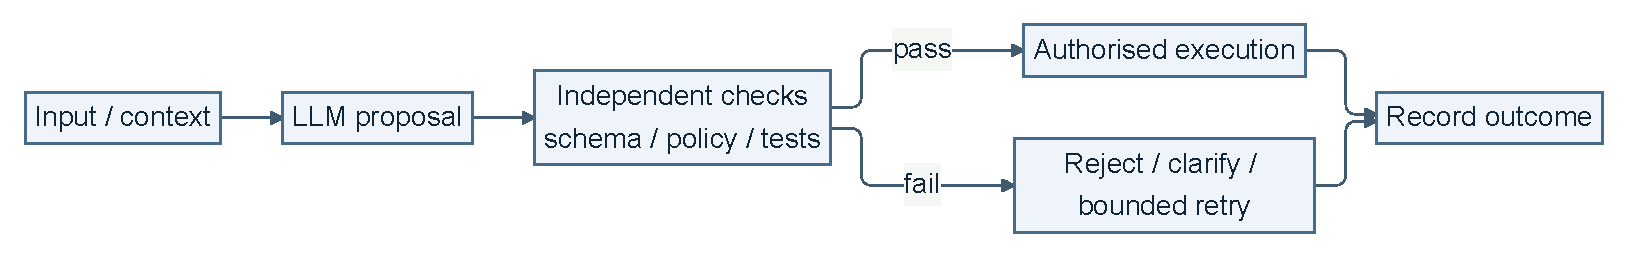
\includegraphics[width=479.32pt]{images/extra-trust.pdf}
\captionof{figure}{LLM outputs need independent checks; generation is not verification}\end{minipage}\par\smallskip

\begin{studycolumns}
\vspace{0pt}



\needspace{4\baselineskip}
\subsection*{16.1 AI engineering vocabulary}
\sectionlabel{h-161-ai-engineering-vocabulary}

\begin{referenceentries}
\textit{\textbf{Term} / \textbf{Definition}}\par\smallskip
\noindent \textbf{\textbf{AI engineering}}: The discipline of \textbf{building, deploying and maintaining AI-powered systems} in the real world; it fuses AI research (what is possible), software engineering (what works reliably) and domain expertise (what matters)\par
\noindent \textbf{\textbf{AI vs ML vs DL}}: AI = broad science of mimicking human abilities; ML = algorithms that improve through experience; DL = multi-layer neural networks for complex patterns\par
\noindent \textbf{\textbf{AI engineering vs ML engineering}}: The guest decks contrast traditional model development/\allowbreak{}training with applications built on foundation models; treat this as a focus distinction, not an exclusive definition\par
\noindent \textbf{\textbf{LLM pipeline}}: Tokenisation \ensuremath{\rightarrow} embeddings \ensuremath{\rightarrow} attention \ensuremath{\rightarrow} next-token prediction \ensuremath{\rightarrow} (training adjusted the weights)\par
\noindent \textbf{\textbf{RAG}}: Retrieval-augmented generation: fetch relevant documents, then generate grounded on them\par
\noindent \textbf{\textbf{Agent}}: Plans and executes a \textbf{sequence of actions} to achieve a goal --- plans across steps, keeps state/\allowbreak{}memory, uses tools, loops until done (vs a stateless, one-shot chatbot)\par
\noindent \textbf{\textbf{ReAct loop}}: THINK \ensuremath{\rightarrow} ACT \ensuremath{\rightarrow} OBSERVE \ensuremath{\rightarrow} THINK \ldots{} with tools, memory, and a \textbf{condition} for termination\par
\noindent \textbf{\textbf{MCP}}: Model Context Protocol --- standard way to expose tools/\allowbreak{}context to models\par
\noindent \textbf{\textbf{Agent risks}}: infinite loops \ensuremath{\cdot} \textbf{indirect prompt injection} \ensuremath{\cdot} \textbf{irreversible actions}\par
\end{referenceentries}
\needspace{4\baselineskip}
\subsection*{16.2 AI failure modes worth remembering}
\sectionlabel{h-162-ai-failure-modes-worth-remembering}

\begin{referenceentries}
\textit{\textbf{Failure} / \textbf{Description}}\par\smallskip
\noindent \textbf{\textbf{Hallucination}}: Confidently stating factually wrong things (e.g. non-existent case citations)\par
\noindent \textbf{\textbf{Bias}}: Amplifying historical discrimination (e.g. a hiring model downgrading r\'{e}sum\'{e}s)\par
\noindent \textbf{\textbf{Prompt injection}}: Malicious instructions hidden in content the model reads (direct vs \textbf{indirect})\par
\noindent \textbf{\textbf{Over-reliance}}: Automation bias --- humans stop checking the output\par
\end{referenceentries}
\textbf{Evaluation challenges:} natural complexity \ensuremath{\cdot} open-ended tasks with multiple valid answers \ensuremath{\cdot} black-box nature \ensuremath{\cdot} benchmark saturation \ensuremath{\cdot} emerging capabilities.

\needspace{4\baselineskip}
\subsection*{16.3 TDD vs BDD vs SDD (the one comparison worth knowing)}
\sectionlabel{h-163-tdd-vs-bdd-vs-sdd-the-one-comparison-worth-knowing}

\begin{referenceentries}
\textit{\textbf{Question it answers}}\par\smallskip
\noindent \textbf{\textbf{TDD} (test-driven development)}: \emph{How do you verify \textbf{one behaviour}?} Write a test first, then code to make it pass\par
\noindent \textbf{\textbf{BDD} (behaviour-driven development)}: \emph{How do \textbf{users/\allowbreak{}business} expect it to act?} Write scenarios in business language, implement against them\par
\noindent \textbf{\textbf{SDD} (spec-driven development)}: \emph{What should the \textbf{system} do?} Write the spec first, implement to match it\par
\end{referenceentries}
\textbf{The SDD loop:} \textbf{Discuss \ensuremath{\rightarrow} Specify \ensuremath{\rightarrow} Delegate \ensuremath{\rightarrow} Evaluate}, with a \textbf{human review checkpoint} for every submitted change. Anti-pattern: \emph{vibe coding} --- vague request \ensuremath{\rightarrow} plausible code \ensuremath{\rightarrow} hope ("fragile \& ungrounded").

\textbf{Mapping back onto SC2006 (the useful part):}


\begin{referenceentries}
\textit{\textbf{SDD phase} / \textbf{SC2006 equivalent}}\par\smallskip
\noindent \textbf{Discuss}: Requirements \textbf{elicitation} (interview/\allowbreak{}workshop, learn the problem domain, name what is out of scope)\par
\noindent \textbf{Specify}: \textbf{SRS} + use case descriptions + data dictionary (the "written spec that survives the session")\par
\noindent \textbf{Delegate}: Implementation (object design \ensuremath{\rightarrow} code)\par
\noindent \textbf{Evaluate}: \textbf{Validation \& verification}, acceptance testing, UAT\par
\end{referenceentries}


\par\smallskip{\color{line}\hrule}\smallskip
\needspace{4\baselineskip}
\subsection*{16.4 AI engineering practice: adapting, evaluating and operating systems}
\sectionlabel{h-164-ai-engineering-practice-adapting-evaluating-and-operating-systems}
The practice deck develops three layers: \textbf{application development} (interface, prompts, context, evaluation), \textbf{model development} (adaptation/\allowbreak{}training, datasets, inference optimisation, evaluation) and \textbf{infrastructure} (compute/\allowbreak{}data management, serving, monitoring).

\begin{itemize}
\item \textbf{Prompt engineering:} specify task, instructions, examples and context. Fast to change; it does not update the model's weights or make unsupported output automatically correct.
\item \textbf{RAG:} retrieve relevant external documents and supply them as generation context. Useful for private or changing knowledge; retrieval quality, latency and document maintenance still matter.
\item \textbf{Fine-tuning:} adapt model weights using suitable labelled examples for a narrow task or desired behaviour. It needs data and training effort; distinguish it from adding context at inference time.
\item \textbf{Evaluation:} use representative tests and quantitative/\allowbreak{}qualitative review throughout development, including component tests and end-to-end behaviour. The Understanding deck also covers fairness, privacy, hallucination, prompt injection and monitoring after deployment.
\item \textbf{Operations:} the practice deck includes REST APIs, containerised dependencies, Kubernetes for orchestration, and CI/\allowbreak{}CD/\allowbreak{}continuous training. Architecture combines the application, model, retrieval/\allowbreak{}data and serving layers; no single tool guarantees quality.
\end{itemize}
The agentic-development deck adds \textbf{automated}, \textbf{observed} and \textbf{human} evaluation evidence: unit/\allowbreak{}integration tests, type checks/\allowbreak{}lint/\allowbreak{}builds; runtime/\allowbreak{}UI behaviour and logs; requirements traceability, diff review, security/\allowbreak{}privacy/\allowbreak{}maintainability. It advocates short feedback loops, enforced checks and searchable structured logs. Passing those checks establishes only what the checks cover, not absence of bugs.

\needspace{4\baselineskip}
\subsection*{16.5 Architecture extension in the Thursday system-design deck}
\sectionlabel{h-165-architecture-extension-in-the-thursday-system-design-deck}
\code{Lecture\_\allowbreak{}12\_\allowbreak{}System\_\allowbreak{}Design\_\allowbreak{}2026\_\allowbreak{}Thursday.\allowbreak{}pdf}, pp. 8--14, discusses intelligence, a three-level capability system (\textbf{foundational, integrative, applied}), LLM agent architecture and brain-inspired agent architecture. These are exploratory architecture examples, not new GES requirements or additional GoF patterns. Their assessment status is not stated in the files.
\end{studycolumns}
